\section{Algorithms}\label{sec:algorithms}
This chapter describes how scalafmt formats Scala code.
We will see that scalafmt's design is inspired by ClangFormat and dartfmt.
However, we believe our design makes a valuable contribution in that it leverages functional programming principles to maximise code reuse and extensibility.

\subsection{Design}
Figure~\ref{fig:architecture} shows an architectural overview of scalafmt.
\begin{figure}
  \centering
  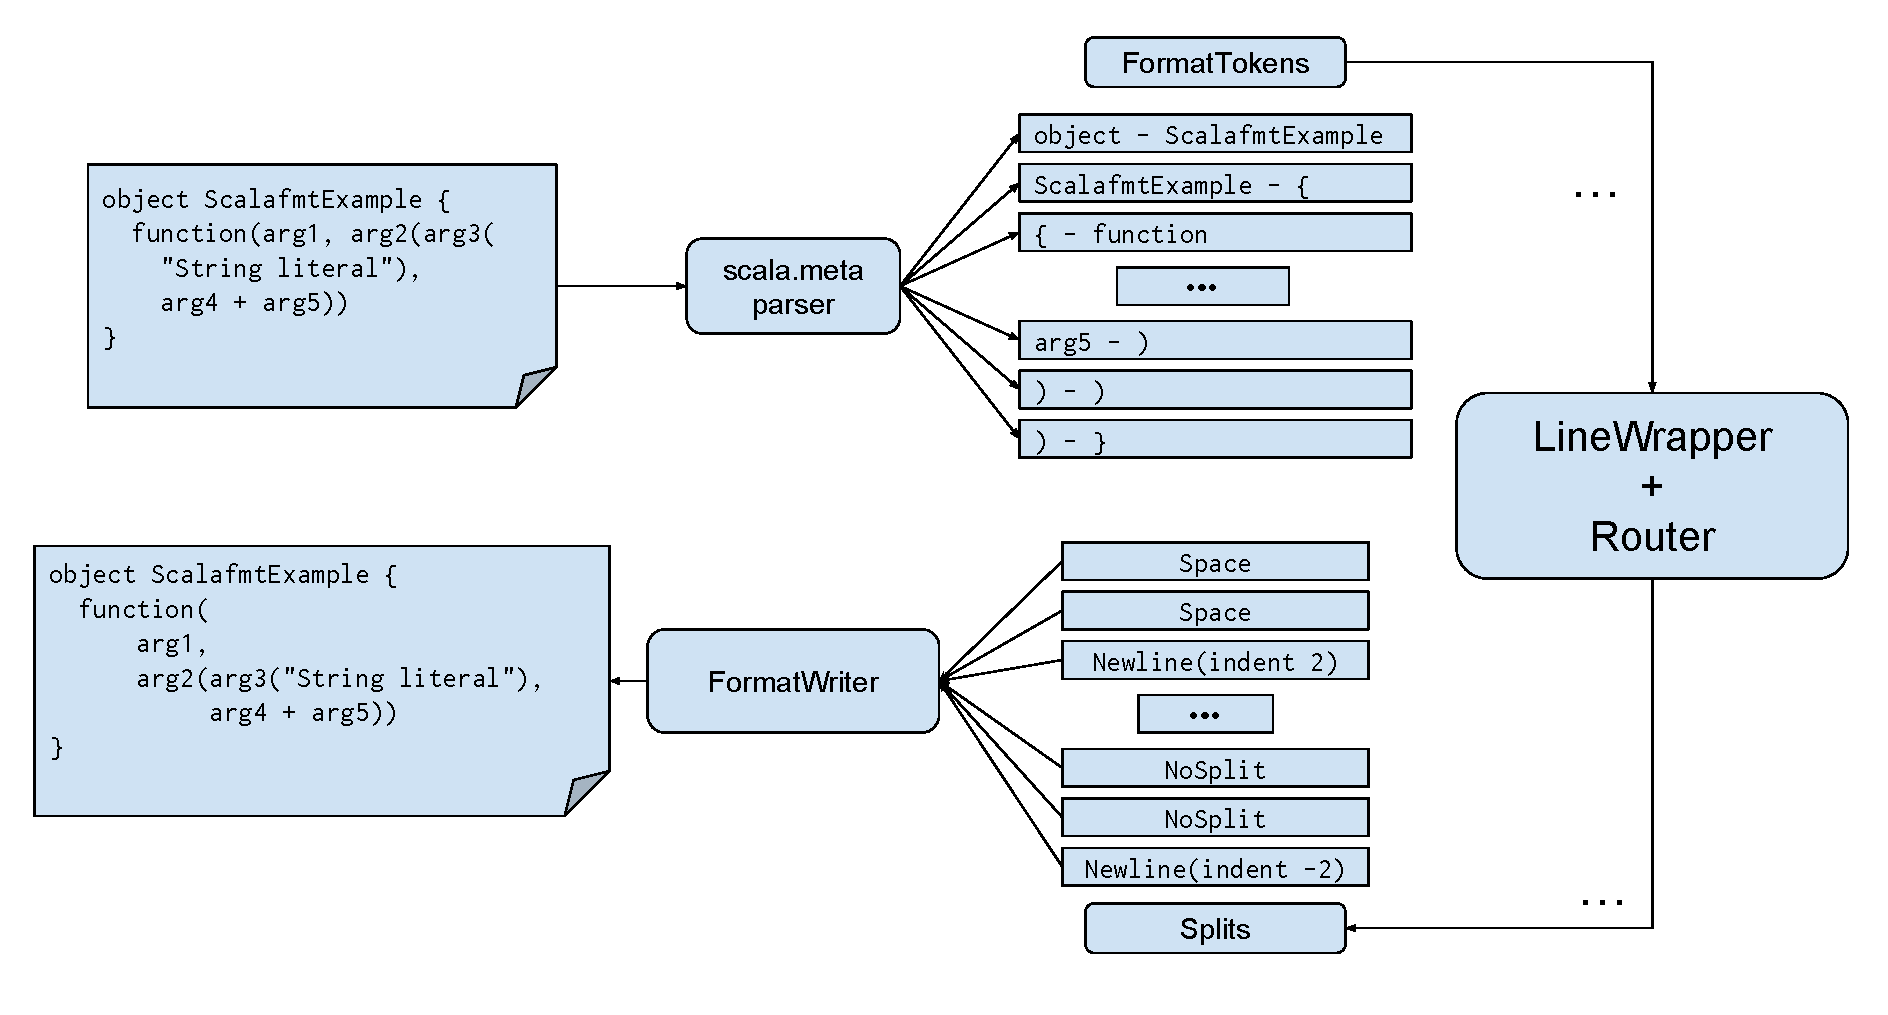
\includegraphics[width=\textwidth]{img/architechture.pdf}
  \caption{Scalafmt architecture}
  \label{fig:architecture}
\end{figure}
First, scalafmt parses a source file using scala.meta.
Next, we feed a sequence of \emph{FormatToken} data types into a \emph{LineWrapper}.
The LineWrapper uses a \emph{Router} to construct a weighted directed graph and run a best-first search to find an optimal formatting layout for the whole file.
Finally, the LineWrapper feeds a sequence of \emph{Split} data types into the \emph{FormatWriter}, which constructs a new reformatted source file.
In the next sections, we explain these data types and abstractions in detail.

\subsection{scala.meta}
Scala.meta\autocite{scala57:online} is a metaprogramming toolkit for Scala.
Many features of scala.meta have made it invaluable in the development of scalafmt.
Most importantly, scala.meta is dialect agnostic, trees preserve all syntactic details in the original file



Scala.meta provides facilities to tokenize and parse a variety of different dialects of Scala, including Scala 2.11, sbt configuration files and Dotty.
Figure~\ref{fig:scalameta} shows how scala.meta parses a simple hello world application in Scala.
\begin{figure}
  \centering
  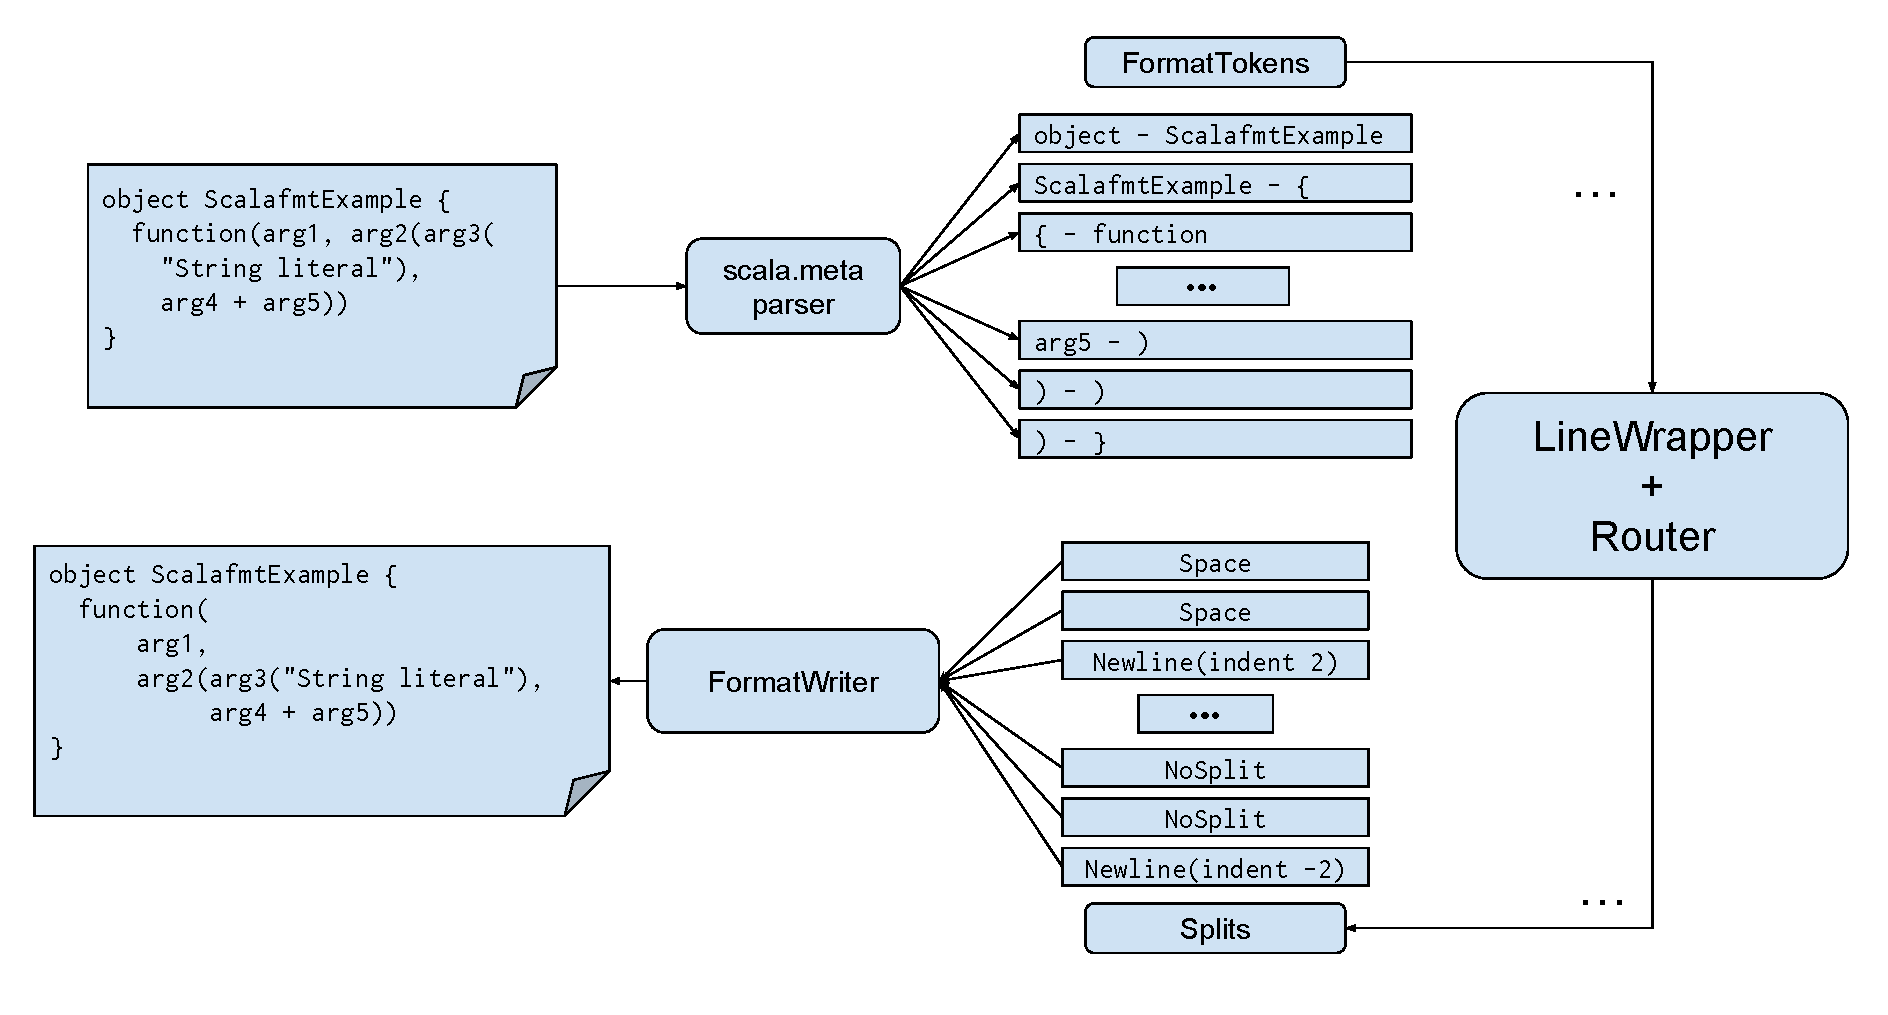
\includegraphics[width=\textwidth]{img/architechture.pdf}
  \caption{Scalafmt architecture}
  \label{fig:architecture}
\end{figure}

A key feature of scala.meta tree node types is that they preserve absolute fidelity of the original source file.
Any syntactic details such as whitespace and comments is attached to each relevant tree node.
Another key feature of scala.meta trees is that tree nodes contain a parent link.
This makes it possible to traverse the 



\subsection{Data structures}
\subsubsection{FormatToken}
\subsubsection{Split}
\subsubsection{Indent}
\subsection{LineWrapper}
\subsubsection{Router}
\subsubsection{Policy}
\subsubsection{OptimalToken}
\subsubsection{State}
\subsection{Optimizations}
\subsubsection{dequeueOnNewStatements}
\subsubsection{recurseOnBlocks}
\subsubsection{escapeInPathologicalCases}
\subsubsection{escapeInPathologicalCases}
\subsubsection{pruneSlowStates}
\subsubsection{FormatWriter}
\begin{itemize}
  \item vertical alignment
  \item comment formatting
  \item stripMargin alignment
\end{itemize}
